\chapter{Systemdesign und Spezifikation}

\begin{figure}[H]
    \centering
    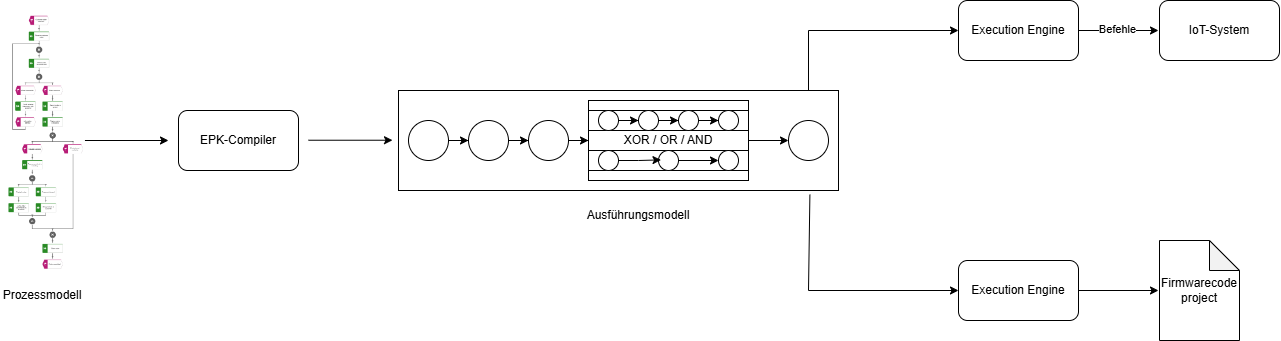
\includegraphics[width=1\textwidth]{Graphics/Systemarchitektur.png}
    \caption{Systemarchitektur}
    \label{fig:systemarchitektur}
\end{figure}

Diese Arbeit setzt ein System bestehend aus einem \textbf{EPK-Compiler} für modellierte EPK-Prozesse in ARIS, welche ein definiertes \textbf{Ausführungdsmodell} liefert,
einer \textbf{Execution-Engine} mit \textbf{Live-Animationsanbindung zu ARIS} und einem \textbf{Codegenerator}, um die Entwicklung der Firmware 
basierend auf dem Ausführungdsmodell zu realisieren.

\section{Architektur und Prinzipien}

Dieses System besteht aus vielen Komponenten, welche sich in ARIS und der ESP-IDF bewegen.

\subsection{Komponenten und Verantwortlichkeiten}

Wie anfangs schon beschrieben hat das System die folgenden Komponenten:

\subsubsection{EPK-Compiler}

Der EPK-Compiler ist dafür zuständig das Prozessmodell in ein Ausführungsmodell zu übersetzen.
Dies geschieht durch Einlesen der Prozesssprache, welche dann in jedem Schritt das Ausführungsmodell Stück für Stück aufbaut.

\subsection{Ausführungsmodell}

Das Ausführungsmodell ist eine Folge an Befehlen, welche die Prozessschritte darstellen. Dabei wird nicht mehr zwischen Ereignis und 
Funktion unterschieden. Dieses Modell ist näher am Programmcode und ein Befehl enthält Metadaten wie Namen und Rückgabetyp. Dieses 
Modell wird dann von der Execution-Engine eingelesen, welche dann die Folge Schritt für Schritt ausführt. Dabei enthält das Modell
auch Kontrollflussstrukturen, welche die Verknüpfungsoperatoren des Prozesses modellieren.

\subsection{Execution-Engine}

Die Execution-Engine nimmt ein Ausführungsmodell an und führt dieses schrittweise auf dem IoT-System aus.

\subsection{Code-Generator}

Der Code-Generator nimmt ein Ausführungdsmodell und generiert Codedateien für das Ziel IoT-System gemäß der einzelnen 
Befehlsschritte.

\subsection{Datenmodelle}
\subsection{Schnittstellen}
\subsubsection{Gegenüberstellung von MQTT und CoAP}

\section{Ausführbarkeit}
\subsection{Ausführungdsmodell auf Basis eines Prozessmodells}
\subsection{Übersetzung des Prozessmodells}
\subsection{Zustandslogik zur Kompilierung des Prozessmodells}
\subsection{Logik zur Ausführung des Ausführungsmodells}

\section{Animation der Automatisierung}
\subsection{Gegenüberstellung von TCP und HTTP}
\subsection{Analogie: WebSockets}

\section{Generierung des Firmwarequellcodes}